\frame{
  \frametitle{Introduction}

  \begin{itemize}
    \item Billiard ball bouncing in a square
    \item Assume no gravity or friction
  \end{itemize}
}

\subsection{Basic Notation}

\frame{
  \frametitle{Basic Notation}
  \begin{definition}
    A table $T \subset \R^2$ is the unit square. Vertical sides are labelled with a $v$. Horizontal sides are labelled with an $h$.
  \end{definition}

  \begin{figure}
    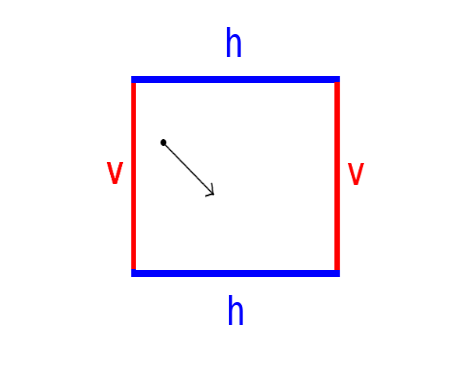
\includegraphics[width=2in]{square_with_sides.png}
  \end{figure}
}

\subsection{Example}

\frame{
  \frametitle{Example}

  \begin{eqnarray*}
    {\color{red}vv}
  \end{eqnarray*}
  \begin{figure}
    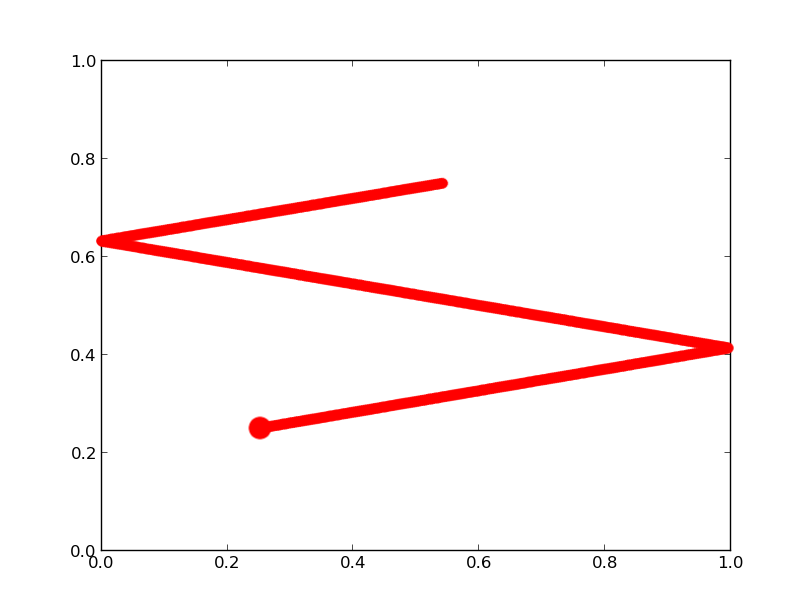
\includegraphics[width=3in]{example/example_1.png}
  \end{figure}
}

\frame{
  \frametitle{Example}

  \begin{eqnarray*}
    vv{\color{red}vhv}
  \end{eqnarray*}
  \begin{figure}
    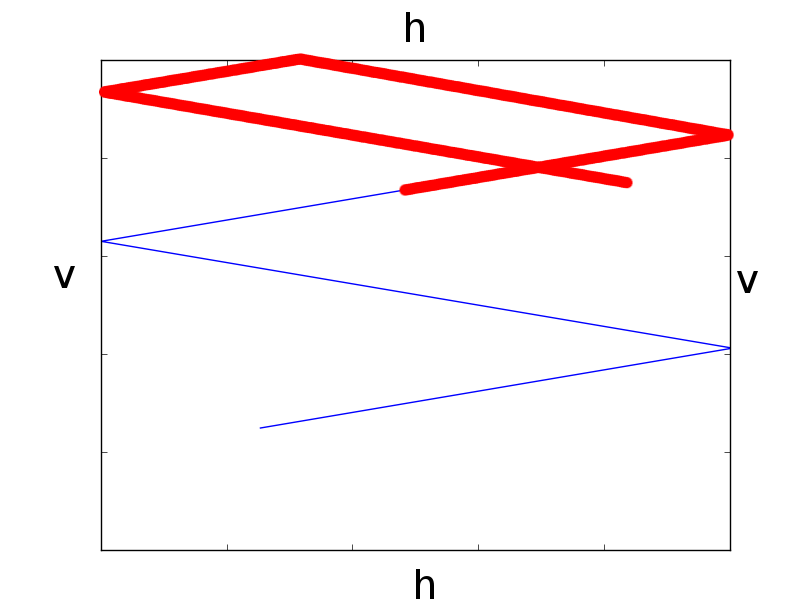
\includegraphics[width=3in]{example/example_2.png}
  \end{figure}
}
\frame{
  \frametitle{Example}

  \begin{eqnarray*}
    vvvhv{\color{red}vvv}
  \end{eqnarray*}
  \begin{figure}
    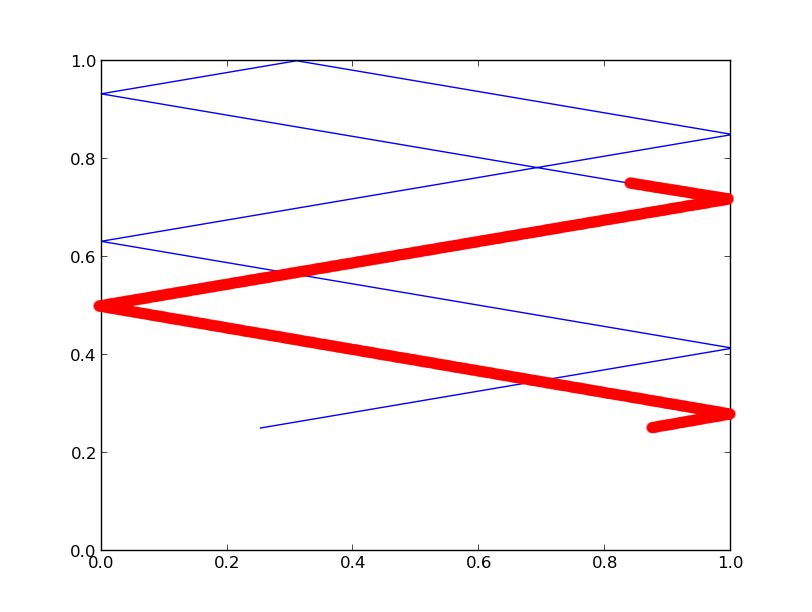
\includegraphics[width=3in]{example/example_3.png}
  \end{figure}
}

\frame{
  \frametitle{Example}

  \begin{eqnarray*}
    vvvhvvvv{\color{red}vhv}
  \end{eqnarray*}
  \begin{figure}
    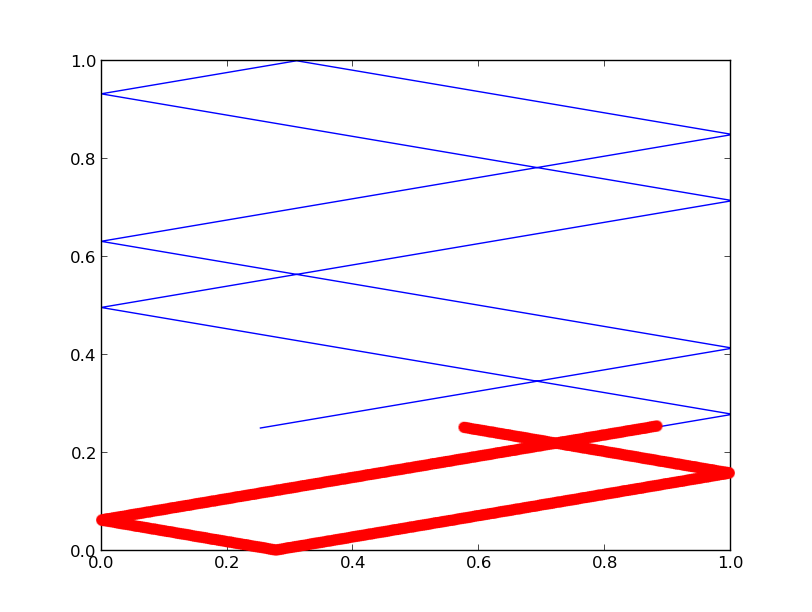
\includegraphics[width=3in]{example/example_4.png}
  \end{figure}
}

\frame{
  \frametitle{Example}

  \begin{eqnarray*}
    vvvhvvvvvhv{\color{red}vv}
  \end{eqnarray*}
  \begin{figure}
    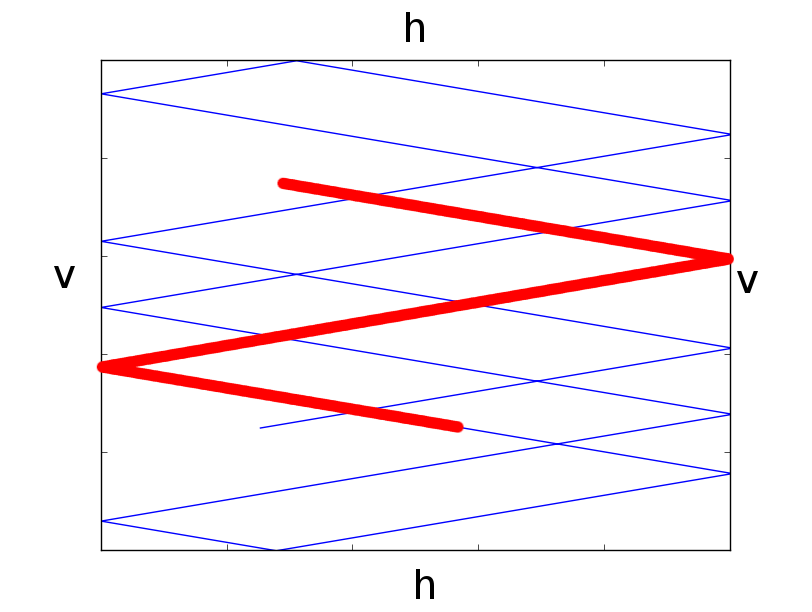
\includegraphics[width=3in]{example/example_5.png}
  \end{figure}
}

\frame{
  \frametitle{Example}

  \begin{eqnarray*}
    vvvhvvvvvhvvv{\color{red}vhv}
  \end{eqnarray*}
  \begin{figure}
    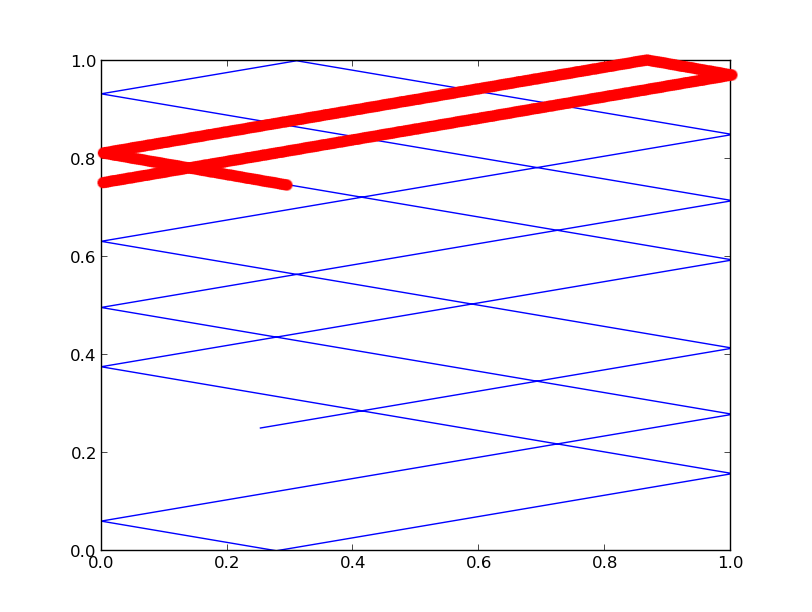
\includegraphics[width=3in]{example/example_6.png}
  \end{figure}
}

\frame{
  \frametitle{Resulting Sequence}
  \begin{eqnarray*}
    vvvhvvvvvhvvvvhv
  \end{eqnarray*}
}

\subsection{Outline}

\frame{
  \frametitle{Presentation Outline}
  \tableofcontents
}

\subsection{Problem Statement}

\frame{
  \frametitle{Problem Statement}

   Problem: Given a sequence of $v$ and $h$ collisions, determine if it is a valid collision sequence.
}

\frame{
  \frametitle{Basic Notation}

  \begin{definition}
    \emph{$v$ collision}: when the ball collides with a $v$ side
  \end{definition}

  \begin{definition}
    \emph{$h$ collision}: when the ball collides with an $h$ side
  \end{definition}

  \begin{definition}
    \emph{Collision sequence ($\alpha$)}: a sequence of $v$ and $h$ collisions which starts and ends with an $h$ collision.
  \end{definition}
}
